\listfiles
\RequirePackage{rotating}
\documentclass[manuscript, screen]{acmart}

% bibliography
% using biblatex isn't very smart because journals are pretty picky. Instead use the default natbib package
% \usepackage[backend=biber,style=trad-abbrv]{biblatex}
% \addbibresource{References.bib}

%\setcitestyle{super,sort&compress}
% \citestyle{acmauthoryear}
\usepackage{booktabs} % For formal tables
\usepackage[ruled]{algorithm2e} % For algorithms
\usepackage{subcaption}
\usepackage[printwatermark]{xwatermark}
\usepackage{xcolor}
\usepackage{graphicx}
\usepackage{tikz}
\usepackage{nameref}

\newsavebox\mybox
\savebox\mybox{\tikz[color=red,opacity=0.3]\node{WORKING DRAFT};}
% \newwatermark*[
  % allpages,
  % angle=45,
  % scale=6,
  % xpos=-35,
  % ypos=30
% ]{\usebox\mybox}

% Metadata Information
\acmJournal{CSUR}
\acmVolume{01}
\acmNumber{01}
\acmArticle{01}
\acmYear{2017}
\acmMonth{07}

%\acmBadgeL[http://ctuning.org/ae/ppopp2016.html]{ae-logo}
% \acmBadgeR[http://ctuning.org/ae/ppopp2016.html]{ae-logo}

% Copyright
% \setcopyright{acmcopyright}
%\setcopyright{acmlicensed}
\setcopyright{rightsretained}
%\setcopyright{usgov}
%\setcopyright{usgovmixed}
%\setcopyright{cagov}
%\setcopyright{cagovmixed}

% DOI
\acmDOI{0000001.0000001}

% some useful shortcut commands
\newcommand{\Pl}{\textbf{Pl}}
\newcommand{\R}{\textbf{R}}
\newcommand{\nisarcomm}[1]{{\color{red} (NRA: #1)}}
\newcommand{\edit}[1]{{\color{blue} #1}}
\newcommand{\hlr}[1]{{\color{red} #1}}

% Document starts
\begin{document}
% Title portion
\title{``I can assure you [\ldots] that it's going to be all right''} 
 \titlenote{HAL 9000, 2001 A Space Odyssey, full quote: ``I know everything hasn't been quite right with me, but I can assure you now, very confidently, that it's going to be all right again.
 }
 \subtitle{A definition, case for, and survey of algorithmic assurances in human-autonomy trust relationships}
 % \subtitlenote{Subtitle note}
\author{Brett Israelsen}
    \authornote{The corresponding author}
    \orcid{0000-0003-1602-1685}
    \email{brett.israelsen@colorado.edu}
    \affiliation{%
        \institution{University of Colorado, Boulder}
        \institution{Department of Computer Science}
        \city{Boulder}
        \country{USA}
    }
    \affiliation{%
        \institution{RECUV}
    }
    \affiliation{%
        \institution{C-UAS}
    }

\begin{abstract}
    As technology become more advanced, those who design, use and are otherwise affected by it want to know that it will perform correctly, and understand why it does what it does, and how to use it appropriately. In essence they want to be able to \emph{trust} the systems that are being designed. In this survey we present \emph{assurances} that are the method by which users can understand how to trust this technology. Trust between humans and autonomy is reviewed, and the implications for the design of assurances are highlighted. A survey of existing research regarding assurances is presented, and several key ideas are extracted in order to refine the definition of assurances. Several directions for future research are identified and discussed.
\end{abstract}


%
% The code below should be generated by the tool at
% http://dl.acm.org/ccs.cfm
% Please copy and paste the code instead of the example below. 
%
\begin{CCSXML}
<ccs2012>
 <concept>
  <concept_id>10010520.10010553.10010562</concept_id>
  <concept_desc>Computer systems organization~Embedded systems</concept_desc>
  <concept_significance>500</concept_significance>
 </concept>
 <concept>
  <concept_id>10010520.10010575.10010755</concept_id>
  <concept_desc>Computer systems organization~Redundancy</concept_desc>
  <concept_significance>300</concept_significance>
 </concept>
 <concept>
  <concept_id>10010520.10010553.10010554</concept_id>
  <concept_desc>Computer systems organization~Robotics</concept_desc>
  <concept_significance>100</concept_significance>
 </concept>
 <concept>
  <concept_id>10003033.10003083.10003095</concept_id>
  <concept_desc>Networks~Network reliability</concept_desc>
  <concept_significance>100</concept_significance>
 </concept>
</ccs2012>  
\end{CCSXML}

% \ccsdesc[500]{Computer systems organization~Embedded systems}
% \ccsdesc[300]{Computer systems organization~Redundancy}
% \ccsdesc{Computer systems organization~Robotics}
% \ccsdesc[100]{Networks~Network reliability}

%
% End generated code
%

% We no longer use \terms command
% \terms{Algorithms, Assurances, Trust}

\keywords{Human Computer Interaction, Trust}

\thanks{This work is supported by C-UAS and Northrop-Grumman Aerospace Systems.}

  % Author's addresses: G. Zhou, Computer Science Department, College of
  % William and Mary; Y. Wu {and} J. A. Stankovic, Computer Science
  % Department, University of Virginia; T. Yan, Eaton Innovation Center;
  % T. He, Computer Science Department, University of Minnesota; C.
  % Huang, Google; T. F. Abdelzaher, (Current address) NASA Ames
  % Research Center, Moffett Field, California 94035.}

\maketitle

% \input{key_ideas.md}
% \input{proposed_framework.md}
\section{Introduction}
    As technology becomes more advanced, those who design, use, and are affected by it in other ways want to know that it will perform correctly, and understand why it does what is does, and how to use it appropriately. In essence, people who interact with advanced technology want to be able to trust it appropriately, and then act on that trust.

    In interpersonal relationships, and otherwise, humans act largely based on trust. For example, a supervisor asks a subordinate to accomplish a task based on several factors that indicate they can trust them to accomplish that task. When consumers make purchases, they do so with trust that the product will perform as promised. Likewise, when using something like an autonomous vehicle, the user must be able to trust it appropriately in order to use it properly.

    With the rapid advancement of the capabilities of intelligent computing technology to do tasks that were previously assumed to be too complicated for computers, there has been much recent discussion regarding how humans can trust this technology -- although the connection to trust is not always made explicit, per se. This discussion has taken place both in public \cite{Spectrum2016-jv,DeSteno2014-cq,Cranz2017-yh,Cassel2017-tn,Danks2017-sb}, business \cite{Banavar2016-nm, Khosravi2016-ke,Moody2017-vd,Rudnitsky2017-in,Benioff2016-tc}, and academic \cite{Groom2007-bz,Lloyd2014-bb,Goodrum_2016-fm,Foley2017-qj,Ghahramani2015-yq,Castelvecchi2016-mr} settings.

    Those who discuss \emph{how} to trust a specific technology are really referring to the need for some indication of the appropriate level of trust to give said technology. In other words, it is desirable to \emph{design} capabilities and methods for intelligent technology which help us achieve appropriate levels of trust in that technology. These capabilities and methods are collectively referred to as \emph{assurances}. %%
    
    Specifically, this survey investigates what assurances an Artificially Intelligent Agent (AIA) can provide to a human user in order to affect their trust. The colloquial definitions of `appropriate use', `assurance', `AIA', and `trust' should suffice for now to give the reader a general idea of the motivation; more formal definitions will be presented in section \ref{sec:background}. It is the author's position that there are many researchers, from different disciplines, who will potentially be interested in this work. This group includes those who are interested in working with, trusting, interpreting, understanding, and/or regulating AIAs.

    Figure \ref{fig:SimpleTrust_one_way} is a simple diagram of the trust cycle that exists between a human user and an AIA (justification for the existence of this cycle will be presented later). Simply, the user's trust is affected by assurances that in turn affect the user's behaviors in interacting with the AIA (e.g. trust AIA with responsibilities, or not). To fully understand and appreciate the importance of assurances, one must have a more formal understanding of each component in figure \ref{fig:SimpleTrust_one_way}. %This is because the cycle is serial, and cannot be complete with any of the components missing. 
This paper provides an overview of the components of figure \ref{fig:SimpleTrust_one_way}. It then turns a more focused attention to assurances, and investigate some of the research that has been done to date. From this survey of literature, properties and classifications of assurances are created, and directions and considerations for further research are presented.

    \begin{figure}
        \centering
        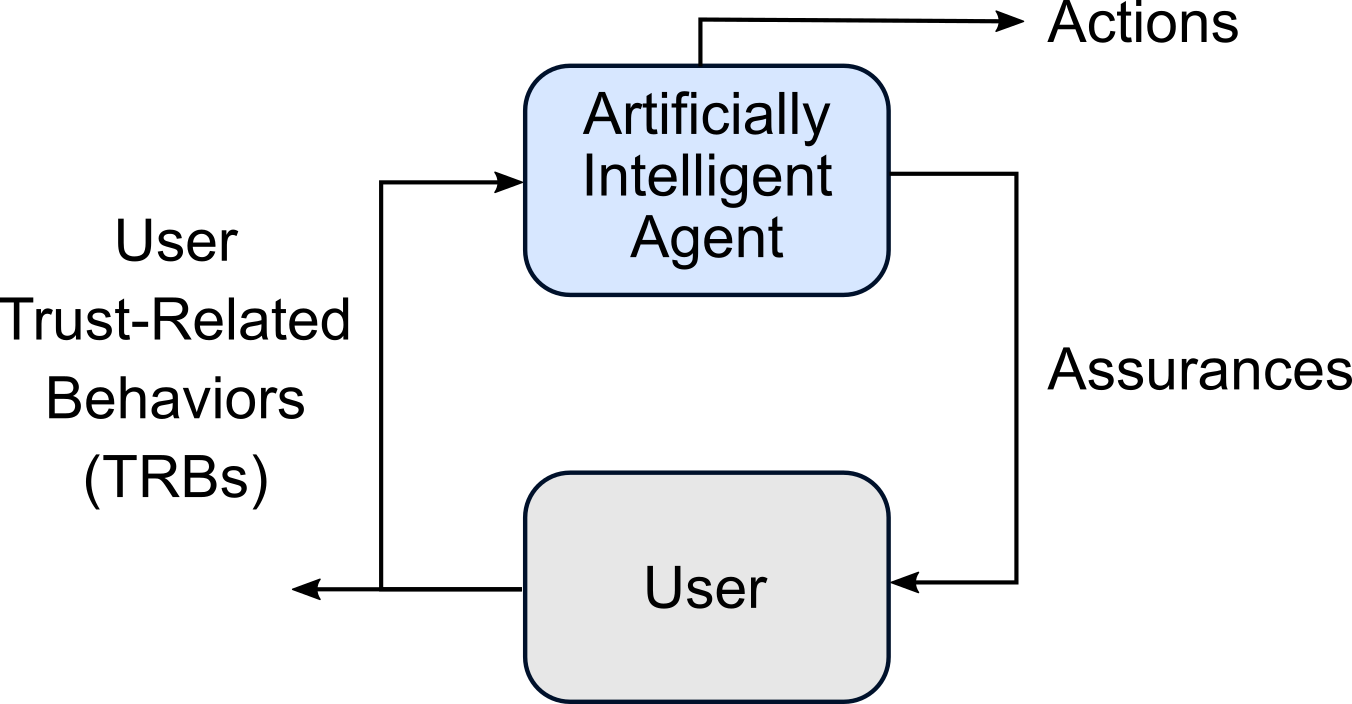
\includegraphics[width=0.7\textwidth]{Figures/SimpleTrust_one_way.png}
        \caption{Diagram depicting the simple one-way trust relationship between a human user and an AIA. Based on a user's level of trust they take certain actions (e.g. give AIA commands), these commands can lead the AIA to certain actions and/or to provide assurances to the user in order to affect their trust.}
        \label{fig:SimpleTrust_one_way}
    \end{figure}

    Some of the novel contributions of this paper include: a detailed description and definition of assurances in general human-AIA relationships; an argument that trust-related behaviors should be used to measure the effect of assurances on user trust; presenting the idea that assurances can be either explicit or implicit; suggestions for promising research directions for explicit assurances.
    % \nisarcomm{This is where the `punchline' and takeaways of this survey should be summarized: i.e. what are the contributions of this work? What are the important arguments to be made? What gaps are being addressed? What is the value of this survey? Who cares about this work? What is interesting/novel about this survey? etc. i.e. what's the point of making the reader read on from here? What's in store for them? Note that this paragraph can be written last, once the remainder of paper is more/less cemented -- but key bullet points should be put in here now/ASAP to build on later}
    To this end, section \ref{sec:background} provides definitions for each of the terms. In section \ref{sec:methodology} I discuss the methodology I used when compiling this survey. Afterwards, section \ref{sec:survey} will discuss the current landscape of assurances that exist in the literature. Finally, section \ref{sec:conclusions} contains some last discussion and conclusions. \nisarcomm{what about Section 5?? -- discuss findings...}

\section{Background and Motivation} \label{sec:background}

\subsection{Motivation}
    Because everyone wants to trust their AIs, whether that be a single classification or regression algorithm, or a more interactive personal assistant that can understand language and communicate. Everyone wants to know how to trust these systems.  

	\begin{sidewaysfigure}[htbp]
        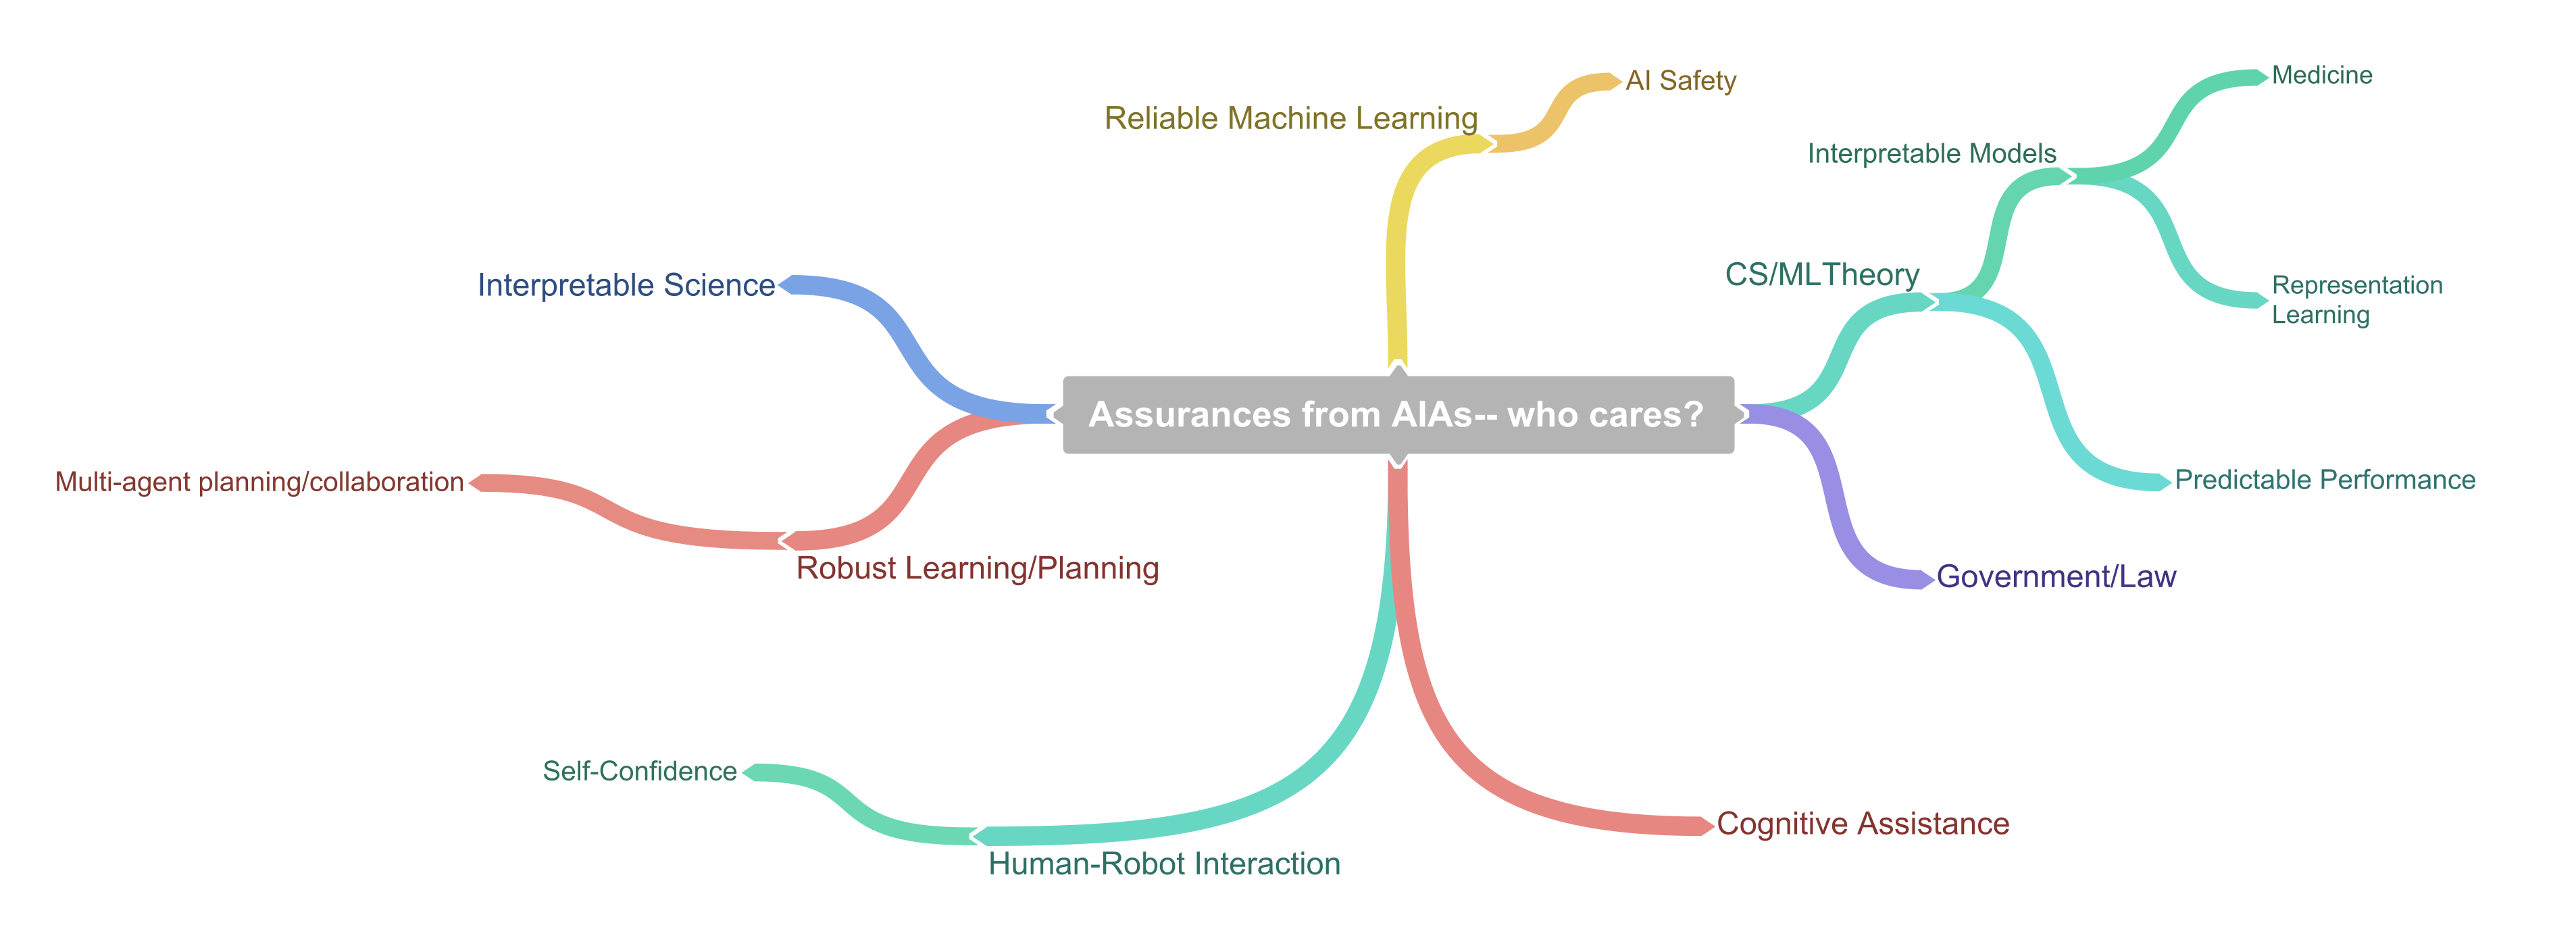
\includegraphics[width=7.5in]{Figures/WhoCares_cleaned}%
    	\caption{A diagram showing some of the academic disciplines that want to trust AIs more fully}
        \label{fig:WhoCares}
    \end{sidewaysfigure}

    \paragraph{Interpretable Science} use data to find causes and insight
    \paragraph{Reliable AI} safety guarantees for robots that have been deployed in real-world environments
    \paragraph{Computer Science} Understand how algorithms will function on real data
    \paragraph{AI/ML} interpret how/why theoretical models function
    \paragraph{Robust Learning/Planning}
    \paragraph{Medicine} understand why data-driven models give predictions
    \paragraph{HCI} help humans and computers interact in a more natural way (where human-human relationships are typically the definition of normal)
    \paragraph{Cognitive Assistance} Ability for user to understand why information was presented
    \paragraph{Government/Law} Regulations on the interpretability of certain algorithms, usage for assistants to lawyers.

    \textbf{Perhaps a table showing the field vs. the AI capability?}, this would help to illustrate the varying needs by fields. Perhaps highlight oversights? \ldots Probably not, we aren't really interested in the different research fields.

\subsection{Artificially Intelligent Agents} \label{sec:aias}
    Intelligent technology spans a wide spectrum of capabilities. With regards to autonomous systems, these might include anything from a thermostat, to the fabled HAL 9000. While the main interest of the authors is geared towards human trust in `advanced' technology, this survey we will take a more holistic view and use the term \textit{Artificially Intelligent Agent (AIA)} to encompass a broad range of technologies that can be considered `autonomous'. This is done in order to provide generally applicable definitions and insights. 

    To this end, an artificially intelligent system needs to possess at least some of the capabilities shown in Figure~\ref{fig:AIcapabilities}~\cite{Russell2010-wv,Nilsson2009-rp,Luger2008-vf}. Some might argue that it is also necessary to add other categories like creativity and social intelligence~\cite{Tao2005-kh}. 
    \brettcomm{SEEMS TO DETRACT---}Some of these categories are also not clearly separable; for instance, where does the capability to `plan' end, and `reasoning' begin? Nevertheless, these capabilities are conceptually useful in defining an AIA:     
    \begin{description}
        \item[Artificially Intelligent Agent (AIA):] an agent that acts on an internally/externally generated goal, and possesses, to some extent, at least one of the capabilities shown in Fig.~\ref{fig:AIcapabilities}.
    \end{description}

	\begin{figure}[htbp]
    	\centering
     	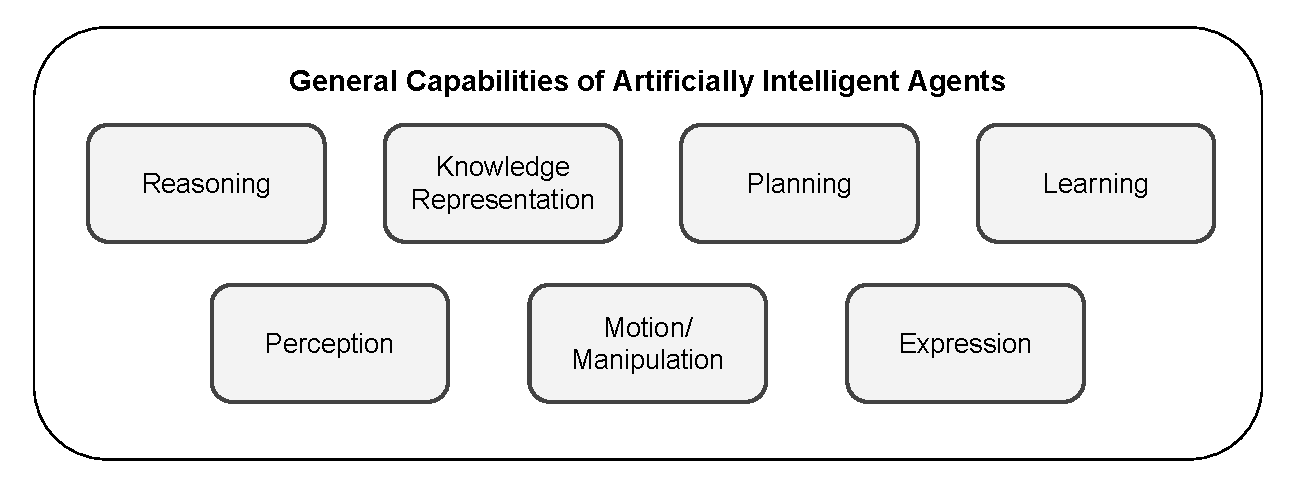
\includegraphics[width=0.55\textwidth]{Figures/AI_capabilities}
    	\caption{List of possible AIA capabilities.}
        \label{fig:AIcapabilities}
    \end{figure}

    The broad range of AIAs implied by this definition is most usefully viewed in terms of scope and adaptability. Scope refers to the range of possible applications for an AIA: does it have a small number of specialized application, or can it be used in many different applications? Adaptability refers to the ability of the AIA to become better at executing its goal over time. Low adaptability has often been associated with `weak AI' whereas high adaptability is often associated with `strong AI'.  Figure~\ref{fig:StrongWeak} depicts these axes for some (real and fictitious) AIAs.

	\begin{figure}[htbp]
    	\centering
     	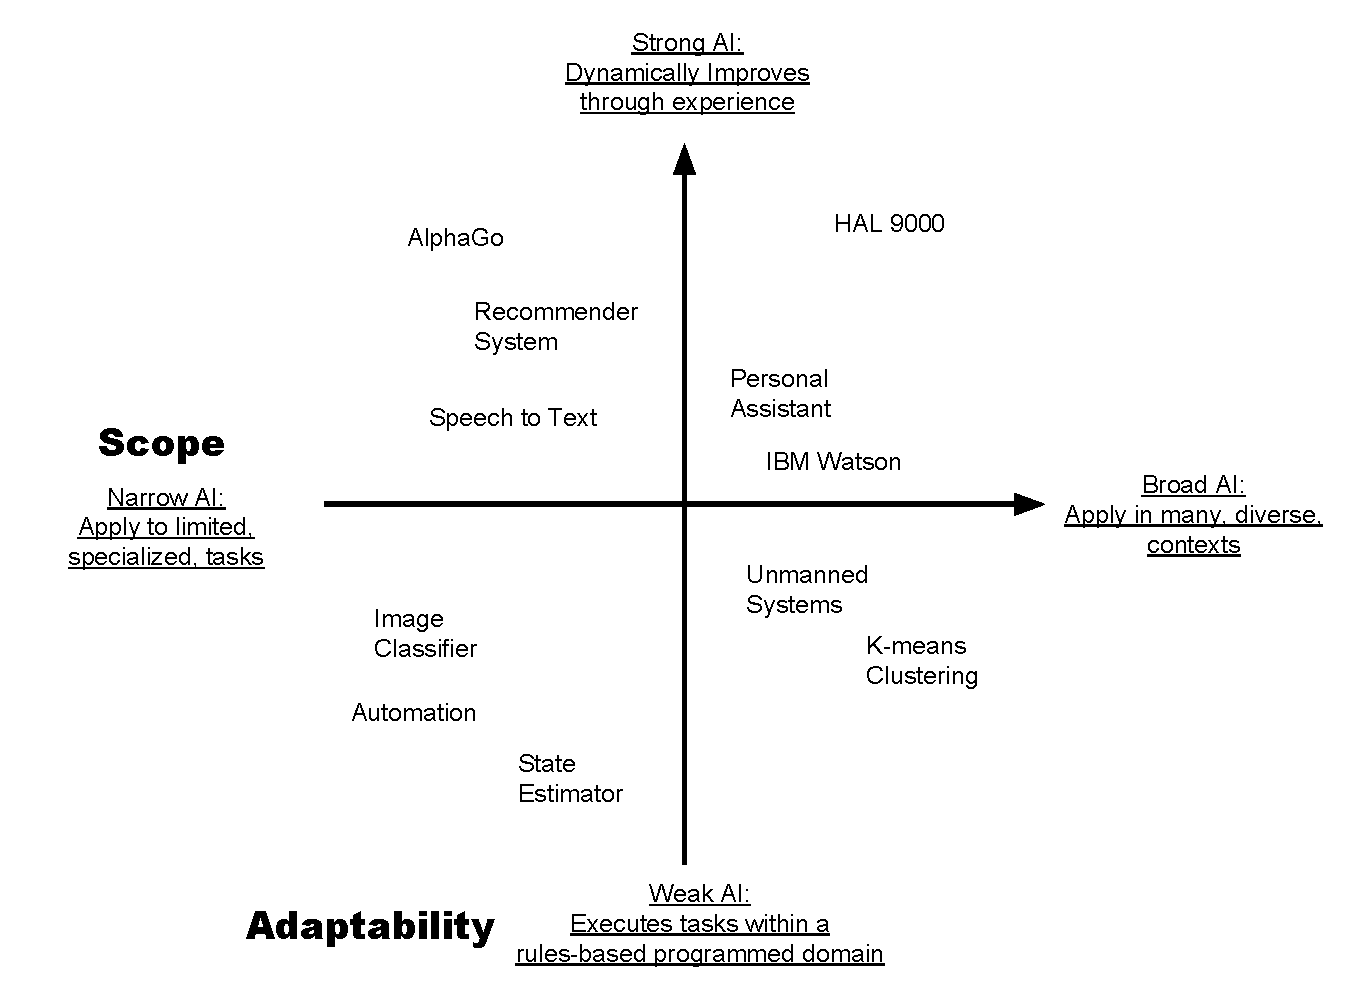
\includegraphics[width=0.7\textwidth]{Figures/strong_weak_narrow_broad.pdf}
    	\caption{Illustration of the range of systems encompassed by the AIA definition. Horizontal axis reflects the scope of the AIA, the vertical axis reflects the adaptability of the AIA.}
        \label{fig:StrongWeak}
    \end{figure}

    Arguably, we might instead have used the term `artificial intelligence' (AI) instead of AIA. However, `AI' carries too much ambiguity (in its fullest meaning, it would possess all capabilities from Figure~\ref{fig:AIcapabilities}, and more). AIA allows the broad inclusion of \emph{any} system in the adaptability/scope plane. The research discipline of machine learning (ML) is a subset of the AI research landscape. Individual ML algorithms might be thought of as being a narrowly scoped AI that is contained within only one of the AIA capabilities. 

    One might also question the need to define AIAs in the first place. This is to aid in the search for and understanding of assurances. As will be shown later, different methods of assurance can be found over the entire range of AIAs, so that an automation system such as a factory robot might be able to use similar assurances -- or more generally, similar principles of assurance -- as might a self-driving car, and vice-versa. The capabilities of AIAs (Fig.~\ref{fig:AIcapabilities}) are the sources of assurances; in other words, assurances cannot exist without some grounding set of AIA capabilities. 

    This definition, while broad, is still useful because it encompasses many of the systems that are typically described as `artificially intelligent'. More importantly, many of the assurances that exist for the simplest AIAs (e.g. chi-square consistency tests for a Kalman filter state estimator) can be adapted/generalized for use in more advanced AIAs. In other words, the proposed definition of AIAs sets an \emph{appropriate scope} for the bodies of research that are likely to have investigated assurances and assurance principles that can be generalized/extended to any intelligent computing system. The definition of AIAs and their range of capabilities also helps to understand and establish what kinds of assurances might be needed in future systems. For example, assurances from an AIA that can only carry out planning tasks will probably differ in design and/or application from assurances from an AIA that can only carry out perception tasks. 

\subsection{User Trust} \label{sec:trust}
    In designing assurances, which affect trust-based user behaviors, it is critical to know what drives those behaviors. Because of this, some time must be spent to understand what trust is. 

    Trust is critical in interpersonal relationships, and it affects the dynamics of \edit{intelligent multi-agent} systems as simple as \edit{one-on-one personal interactions}  \cite{Lewicki2006-hj}, to more complicated ones such as financial markets and governments \cite{Fukuyama1995-un}. Consequently, researchers in psychology, sociology, and economics have historically sought to understand the fundamental principles of trust, each with the aim of understanding their field better \cite{Gambetta1988-pi}. Moral philosophers have also thought intently about the topic \cite{Baier1986-im}.

    Due to wide interest spanning many disciplines it is difficult, if not impossible, to write a succinct definition of trust that would appease all interested parties. Besides that, trust is actually a very broad concept that evades precise definitions at a high level. However the following definition, adapted from \cite{McKnight2004-vv}, is broad enough to avoid too much contention:

    \begin{description}
        \item [Trust:] \edit{a psychological state in which an agent} willingly and securely becomes vulnerable, or depends on, a trustee (e.g., another person, institution, or an AIA), having taken into consideration the characteristics (e.g., benevolence, integrity, competence) of the trustee.
    \end{description}

    \subsubsection{Trust in AIAs and humans?}
        Trust is generally understood to exist between people. Is it possible for a human to enter into a trusting relationship with an AIA?
        % In their paper regarding important human factors that should be considered when designing autonomous machines \cite{Sheridan1984-kx} are seemingly the first to discuss the idea that trust relationships between humans and autonomous systems are important, and to suggest that humans need some assurance that the ``commands will be carried out properly''. They also mention the idea that ``there needs to be an accurate perception of [the autonomous system's] trustworthiness''. Finally they suggest that ``appropriate criteria for trust need to be studied to develop a theory of trust in supervisory control''.
        % Perhaps motivated by \citeauthor{Sheridan1984-kx}\cite{Sheridan1984-kx}, a few years later \cite{Muir1987-mk}, and later in more detail \cite{Muir1994-ow}, create a psychologically based model of trust that considered the ``component expectations of trust'' of \cite{Barber1983-yc} and the dynamic evolution of trust from \cite{Rempel1985-sg}, to make a framework for studying trust in human-machine relationships.
        % \citet{Muir1996-gt} reported the results of two experimental studies to investigate the validity of her proposed model. She claims that these were the first experiments to explicitly ask "operators to rate their trust in automated equipment", and to see if they could do so under normal operating conditions. She found that operators were able to rate their trust in the automation, and that the level of trust changed based on different performance characteristics of the automated system. In her own words: "These results suggest that operators' subjective ratings of trust and the properties of the automation which determine their trust, can be used to predict and optimize the dynamic allocation of functions in automated systems".
        That humans actually do feel trust towards machines has been experimentally confirmed several times in research using common subjective psychological questionnaires. Some examples include: \citet{Muir1996-gt,Reeves1997-ad,Groom2007-bz,Mcknight2011-gv,Riley1996-qm,Bainbridge2011-pl,Kaniarasu2012-mo,Salem2015-md,Desai2012-rc, Freedy2007-sg, Wang2016-id, Inagaki1998-cl, Kaniarasu2013-ho}. 
\nisarcomm{This next part is worth mentioning:} Several academic experiments have investigated the possibility of trust existing between humans and (according to the terminology of this survey) AIAs. All found that some level of trust can be formed in such relationships. For instance, ref. \citet{Lacher2014-yc} points out that people trust an AIA at different levels. For example, an operator would have different perspectives on trust based on their level of interaction with the AIA. The designer of an AIA would also trust the AIA differently than an end user, due to the differing nature of the trust relationship from one to the other. 
        % \citet{Lankton2008-ct} claims, and finds some support for the idea, that trust in technology is fundamentally different from interpersonal trust between humans. They demonstrate the validity of the hypothesis by using a survey of 427 college students regarding Facebook. However, the authors point out that this study was based on a single set of survey data about facebook, and may not be unbiased or apply to other technologies. Beyond this, it is the author's opinion that the `fundamental differences' they point out are not that divergent from the human-human trust model.

        Ref. \citet{Tripp2011-cq} investigate the variation of trust between humans and different levels of technology. They run experiments with three different levels of technology: Microsoft Access, a recommender system, and Faceobook. They found that `human-like' trust applied more to Facebook, while `system-like' trust applied more to MS Access. They conclude that if the system is `human enough', then a human trust model is appropriate. However, the authors also caution that it is important to check first \nisarcomm{Check what first???}.

        Given this research, we will take the position of presenting a human-human trust model and using it as a basis for human-AIA trust -- with the understanding that the applicability of the model varies with the complexity of the AIA. For example, something in the lower-left quadrant of \ref{fig:StrongWeak} \edit{?????} to the upper-right quadrant. \nisarcomm{CAREFULLY READ ALOUD WHAT YOU ARE WRITING: (i) previous sentence is a sentence fragment, and (ii) also this seems like a very strange thing to say: you are applying a human-human trust model as basis for all human-AIA trust, but then you are immediately disclaiming that it is not really applicable in all AIA cases? Then why bother presenting it?! Are you really trying to say something else here, i.e. some features of the model may be more important than other features depending on where you are on the spectrum of adaptability vs. capability? }

\subsubsection{A Model of Human-AIA Trust}
We now present a model of human-AIA trust, which will cast insights on assurances that will be discussed later. It should be noted that this model is being presented as \emph{one possible model} that can be helpful in understanding assurances -- it is neither the only model nor a perfect model. As research advances, such models will also likely continue to evolve, and the ideas of assurances will naturally evolve as well.
        % This has been recently attempted in the context of human-AIA relationships \cite{Lahijanian2016-nd}, but with an overly simplistic reduction of trust. The reality is that trust is extremely complex, and so dealing with it in the setting of human-AIA relationships is going to be complex.

In work relating to business management, McKnight in ref. \citet{McKnight1998-ty} and later in ref. \cite{McKnight2001-fa} performed what is, arguably, the first multi-disciplinary survey and unification of trust literature, which also condensed it into a single typology. The resulting model is shown, with some minor adaptations, in Figure \ref{fig:UserTrust}.

        \begin{figure}[htbp]
            \centering
            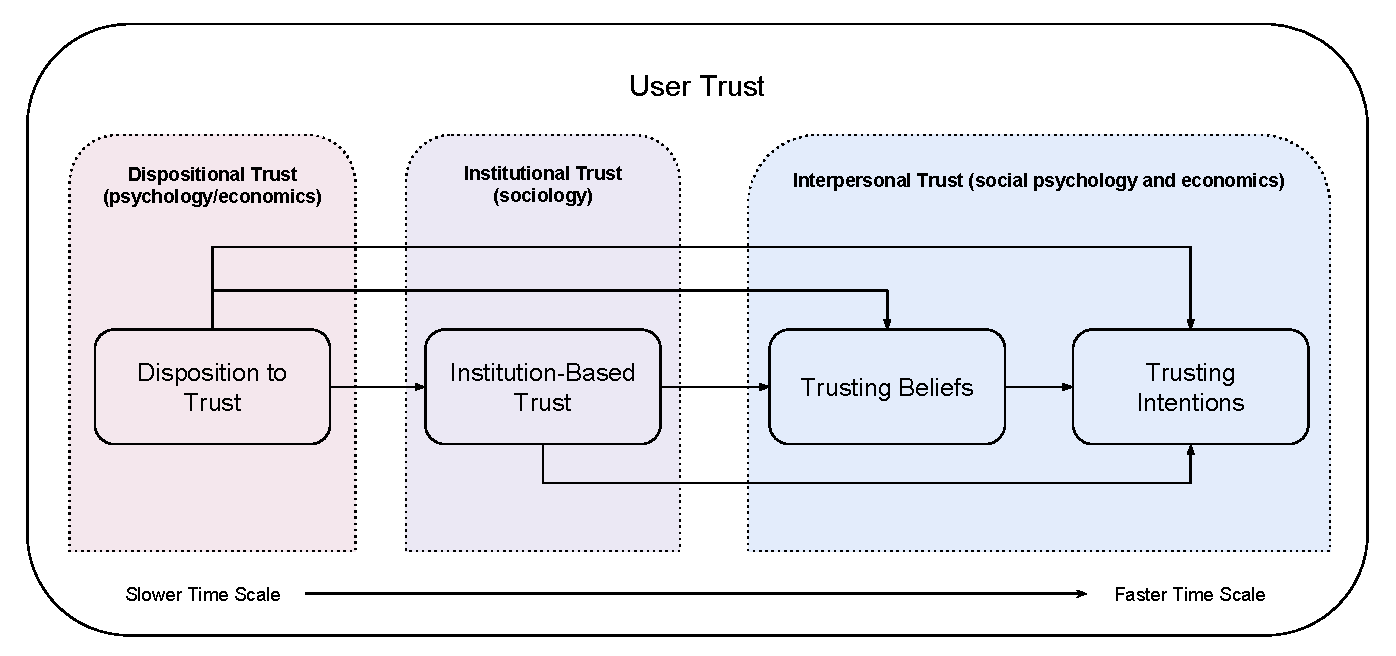
\includegraphics[width=0.9\textwidth]{Figures/UserTrust}
            \caption{Interdisciplinary trust model proposed by \citet{McKnight2001-fa}. The three main categories are delineated, and corresponding disciplines that are interested are listed within parentheses. Connections indicate a causal relationship.}
            \label{fig:UserTrust}
        \end{figure}

        The categories \nisarcomm{of what??} are defined as follows: \nisarcomm{You jumped into the figure without describing anything about it at a high level at all!!! What categories are you talking about -- categories of WHAT exactly??? SAY what the figure means at a high level -- walk the reader through it so they are on the same page as you -- \textbf{DON'T WRITE TO YOURSELF, WRITE FOR YOUR AUDIENCE (WHICH HAS NOT YET SEEN WHAT YOU HAVE SEEN) -- PUT YOURSELF IN AUDIENCE'S SHOES}}

        \begin{description}
            \item [Disposition to Trust:] The extent to which one displays a consistent tendency to be willing to depend on others (and AIA) in general across a broad spectrum of situations and persons
            \item [Institution-Based Trust:] One believes that regulations are in place that are conducive to situational success in an endeavor
            \item [Trusting Beliefs:] One believes that the AIA has one or more characteristics beneficial to oneself
            \item [Trusting Intentions:] One is willing to depend on, or intends to depend on, the AIA even though one cannot control its every action
        \end{description}

        Each of these main categories \edit{of trust} has components defined in Figure \ref{fig:Assurance_classes}. These components were defined through the compilation of many research studies across research disciplines, and because of this represent the most accurate notion of the components of trust available. \edit{It is asserted here} that these trust components \hlr{describe the possible dimensions that constitute trust-related behaviors} \nisarcomm{this is not worded correctly -- these are components of trust, not trust-related behaviors -- they might inform TRBs, but they are not in and of themselves things that constitute TRBs (which you have yet to define at this point!)}, and at which assurances \hlr{must be} targeted. \nisarcomm{MUST be targeted? or are targeted? i.e. is there any real choice? }

        \begin{sidewaysfigure}[htbp]
            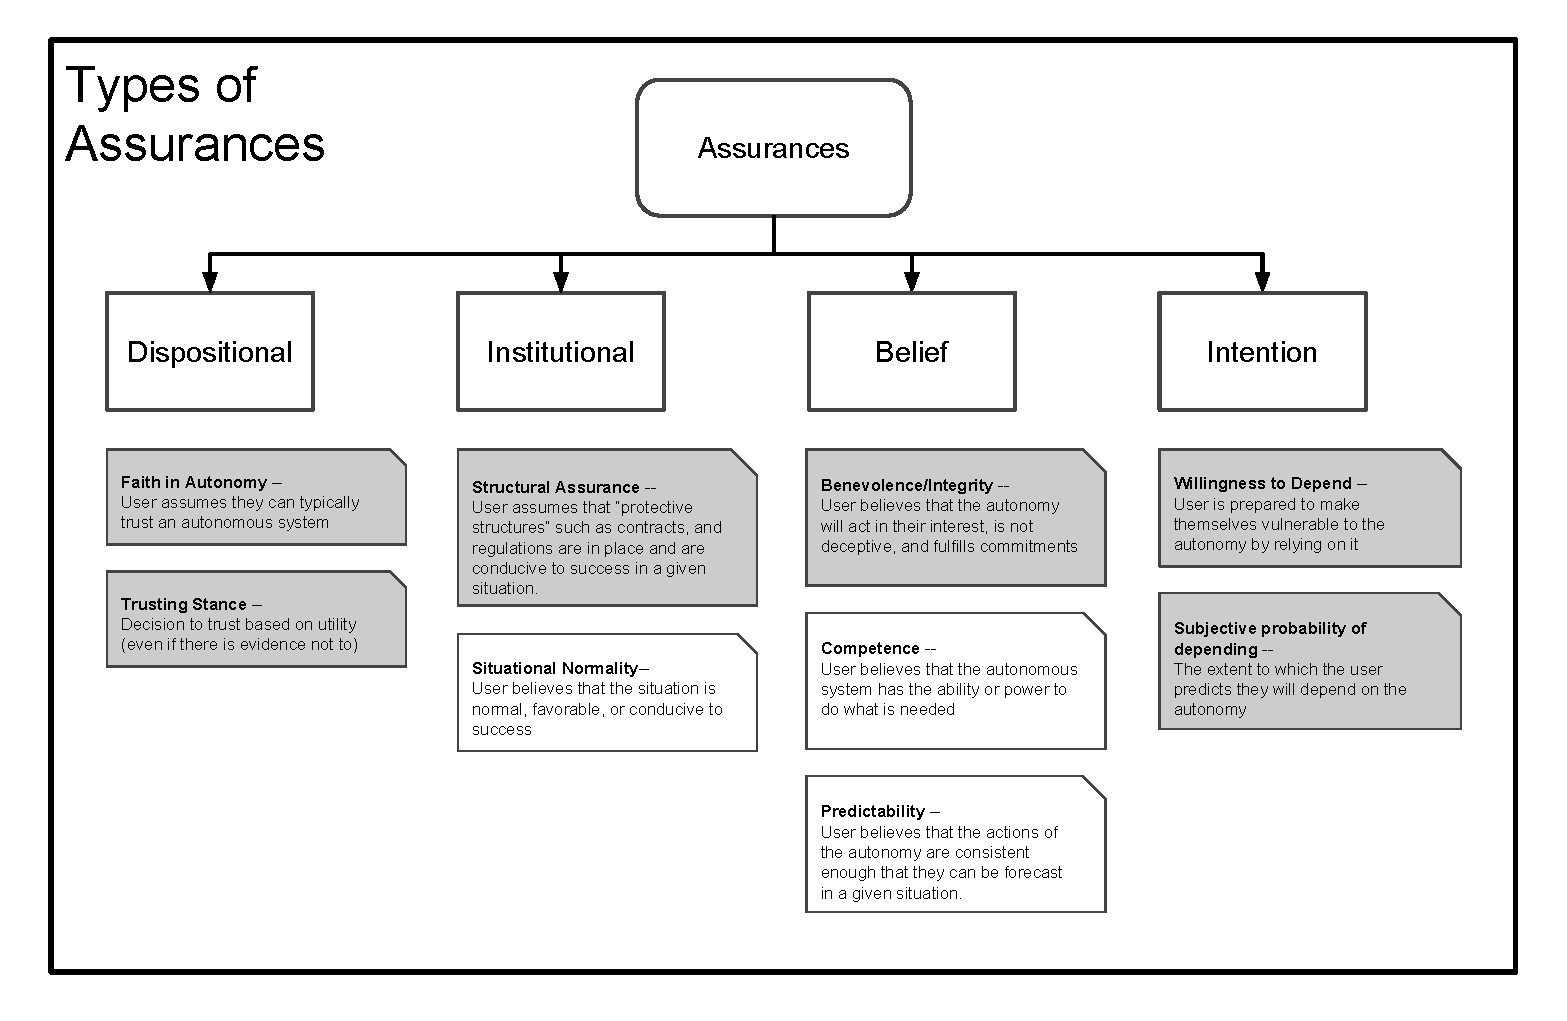
\includegraphics[width=8in]{Figures/Assurances.pdf}%
            \caption{\textbf{Diagram delineating the possible classes of assurances, and suggesting those classes that directly apply in calibration of TRBs \ldots obviously needs to be finished \ldots}}
            \label{fig:Assurance_classes}
        \end{sidewaysfigure}

%trbs.tex
%\nisarcomm{trim, merge, move earlier?....}

%Researchers of all disciplines widely accept that 
Trust ultimately leads to some kind of meaningful behavior or action which reflects the level of trust \cite{Lewis1985-pr}. 
%; this idea was highlighted by \citet{Lewis1985-pr}.  
These are called `trust-related behaviors' (TRBs) \cite{McKnight2001-fa}. %, which is the term that will be used in this survey. 
In the case of a human-AIA relationship per Fig. \ref{fig:SimpleTrust_one_way}, %and \ref{fig:RoadNet}, 
Some example TRBs could include the kinds of tasks the human user assigns to the AIA, accepting and following through on a plan produced by the AIA, or directing that a new plan be made, or switching off autonomous capabilities altogether to teleoperate and perform tasks manually through a physical mechanism that the AIA otherwise controls.  %the vehicle. 

%\subsubsection{Calibration of Trust-Related Behaviors}
    
    Trust is not a univariate quantity that can be objectively measured. Rather, it is a multidimensional phenomenon whose `relative magnitudes and directions' must be observed through changes in TRBs, or qualitative self-reports reported in surveys \cite{Muir1996-gt}. It thus comes as no surprise that TRBs are the more objective measure due to the fact that people are not always consistent in their ratings, and may sincerely feel different levels of trust while performing similar TRBs. \citet{Parasuraman1997-co} were interested in understanding the use of automation by humans, and defined terms to describe that use. Here it is proposed that, by extension, those terms also apply to the behaviors of humans towards more advanced AIAs. Within this scope the definitions are as follows: \textit{Misuse:} over-reliance on an AIA (which could manifest itself in a user's unrealistically optimistic expectations of performance); \textit{Disuse:} under-utilization of an AIA (e.g. a user turning off the AIA, or failing to use all of its capabilities); \textit{Abuse:} Inappropriate application of an AIA (where \emph{application} in this case means the choice to deploy an AIA in a certain context).

    \nisarcomm{can trim down this parag a bit...}
    Following Fig.~\ref{fig:SimpleTrust_one_way}, an AIA's assurances are ideally designed to steer the user away from misuse, disuse, or abuse of the AIA, i.e. towards otherwise appropriate TRBs. This can only be done by properly `calibrating' assurances to suitably influence user trust. This is a point that, to some extent, has been informally mentioned in \cite{Muir1994-ow,Lillard2016-yg,Lee2004-pv,Hutchins2015-if}. Note that other researchers who propose `calibration' (or other similar concepts) often suggest calibrating \emph{trust} as opposed to TRBs. \citet{Dzindolet2003-ts} found that providing system performance feedback tended to increase user's \textit{self-reported trust}, even though user's resulting TRBs did not reflect self-reported trust levels. This shows the danger of calibrating `trust', as opposed to calibrating the TRBs. 
    TRB calibration focuses on concrete and measurable behaviors that are universally applicable. 
    In contrast, trust calibration involves influencing a quantity that is directly immeasurable, and that, when measured indirectly, is subject to individual human differences and biases. 
\subsection{Assurances} \ref{sec:assurances}
    The term assurances was introduced in the previous section as the name by which feedback will be known in a human-AIA trust relationship. As assurances are the main topic of this paper, and are have received very little attention in trust literature, a more detailed definition and discussion is merited.

    \citet{McKnight2001-fa} allude to this kind of feedback in an e-commerce relationship as `Web Vendor Interventions' and mention some possible actions that might be used in that specific application. They go as far as making a diagram that indicates that these interventions could affect the `Trusting Beliefs', `Trusting Intentions', and `Trust-Related Behaviors' (see Figure \ref{fig:UserTrust}).

    \citet{Corritore2003-gx} refer to assurances as `trust cues' that can influence how online users trust vendors in an e-commerce setting. \citet{Lee2004-pv} discuss `display characteristics', which are methods by which an autonomous can communicate information to an operator.
    
    The term assurances is perhaps earliest used in the context of human-automation relationships by \citet{Sheridan1984-kx}. More recently, and formally, \citet{Lillard2016-yg} defined the term `assurance', I extend the definition to be more general
    
    \begin{description}
        \item [Assurance:] A property or behavior of an AIA that affects a user's trust. As used here, the term is not intended to have a positive or negative connotation -- assurances can decrease trust.
    \end{description}

    Most familiar with the fields of AI, ML, data science, and robotics will recognize terms like \emph{interpretable}, \emph{comprehensible}, \emph{transparent}, \emph{verified and validated}, \emph{certified}, and \emph{explainable AI}, with respect to the models or performance of a designed system. A key claim of this paper is that from a high level all of these terms have the same aim: for a user to be able to trust an AIA to operate in a certain way, and based on that trust behave appropriately towards the AIA. Those actions might include re-design, as well as adjusting TRBs.
%
    % Assurances and `interpretability' are delicately linked. In fact, interpretability would be classified as one embodiment of an assurance. This relationship is highlighted by \citet{Vellido2012-nm} where they illustrate that interpreting an AIA is part of the knowledge discovery process.

    The sections that follow outline different classes of assurances.

    \subsubsection{Source-Target Classification}
    It is convenient to refer to assurances by way of their source and target. Intuitively, there may be a set of different algorithms that are useful for making assurances that convey information about planning to the competence dimension of the user's trust. It is easier to refer to these assurances in terms of their source and target. So, for this example that class of algorithms would be the `planning-competence' class.
    
    Not only is this useful shorthand for communicating about the purpose of the algorithms, but it is useful in classifying the range of assurance algorithms that exist. There may also be a class of algorithms that span multiple source-target capabilities. For example there may be a kind of algorithm that can give a `learning-competence' assurance, as well as a `planning-competence' assurance.

    This is especially true since many of the AIA capabilities can overlap. Also, the effects of assurances cannot be guaranteed to affect only one trust dimension.

    Figure \ref{fig:Assurance_classes} shows the hierarchy of proposed assurance classes. The categories mirror those of the trust model proposed by \citet{McKnight2001-fa}, but with the emphasis on what an AIA has the ability to most readily influence (and consequently where most research is found). The boxes with the beveled corner identify and define the different classes of assurances. All classes are included here for completeness and generality. Although, while it is hypothetically possible for an AIA to influence a persons general `Trusting stance' given enough time\footnote{One might imagine an AIA that specifically speaks to the human about the benefits or drawbacks about trusting even though there might not be evidence to do so, similar to the role a counselor might play}, the gray boxes are not considered further in this survey, as practically no direct research exists in the realm of human-AIA relationships.

    \textbf{ugggg, this gets a little complicated, but it's not supposed to be}.

    \subsection{Component and Composite Assurances}
Assurances can be either component or composite. This was seen a little through the survey. The definitions are as follows:

\begin{description}
    \item [Component:] An assurance that originates from a single AIA capability source, and targets a single trust dimension target.
    \item [Composite:] The combination of more than one component assurance into a single assurance. 
\end{description}

\begin{figure}[!htbp]
    \centering
    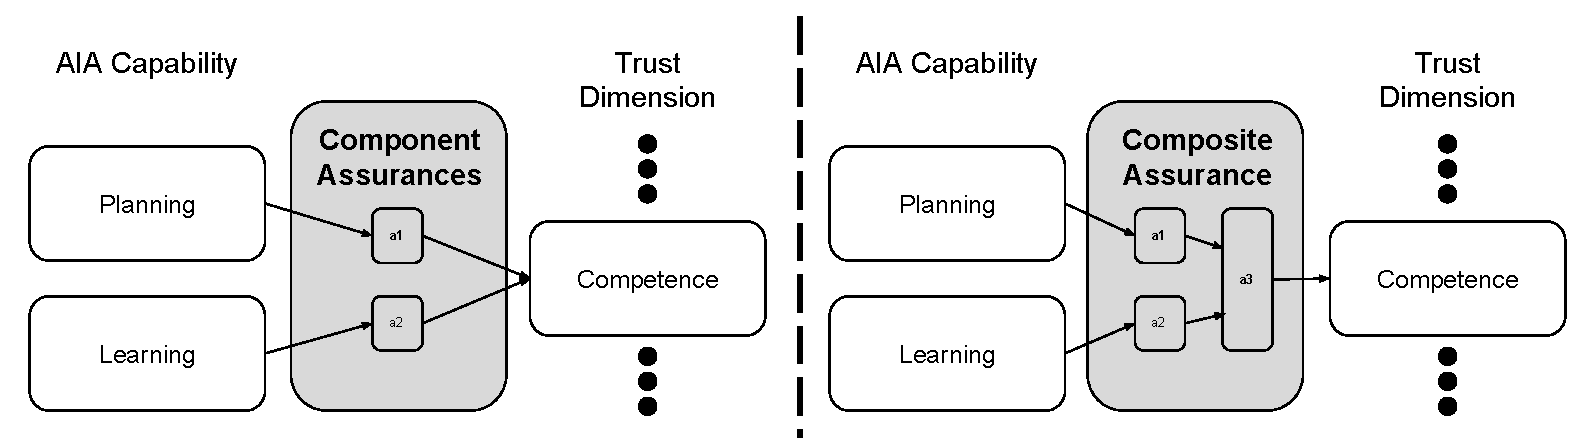
\includegraphics[width=0.9\textwidth]{Figures/Assurance_component_composite.pdf}
    \caption{Figure illustrating the difference between component and composite assurances. The existence of multiple assurances does not imply a composite assurances, rather the combination of multiple component assurances into a single assurance constitutes a composite assurance.}
    \label{fig:assurance_mapping}
\end{figure}

Figure \ref{fig:assurance_mapping} illustrates the concepts of component and composite assurances.

\paragraph{Component Assurances:} Component assurances are perhaps the most well researched in the existing literature. This is likely because several verified component assurances are the predecessors to composite ones. A component assurance might include displaying the confidence of a classification prediction, or visualizing a model as discussed in section \ref{sec:q2}.

\paragraph{Composite Assurances:} Composite assurances are assurances that are built of several components. A notable example is the work by \citet{Aitken2016-cv} who propose a measurement called `self-confidence', applicable to Partially Observable Markov Decision Processes (POMDPs). This metric combines five component assurances into a single composite assurance that is meant to distill the information into a value that a novice operator could understand easily. This paper was discussed in more detail in \ref{sec:q2}. 

    \emph{Tutoring vs Telling:}
Most assurances investigated to date are `telling', in that they do not consider the experience or other traits of different users. The ability to adapt to different users, and to tutor them to appropriate trust will become more critical as time passes due to the diversity of users bases for advanced AIAs and time that users will interact with them. A tutoring assurance would be a planned, dynamic, sequence of assurances that would change in time to adapt to the user's needs. This might include modification of assurances to help a user avoid boredom, or to use the system differently in varying circumstances. It isn't surprising that, to our knowledge, no research has been done with respect to tutoring a user in a trust relationship. This is a complex problem to address that would involve understanding how different users learn, and what an appropriate strategy would be to teach them to have appropriate TRBs. However, a rich resource (not investigated in this paper) would be the work on tutoring systems \citet{Wenger2014-ld} and algorithmic teaching \citet{Balbach2009-jw}.

    \subsubsection{Explicit and Implicit Assurances}
\citet{Sheridan1984-kx} briefly alluded to the existence of explicit and implicit assurances when they discussed the nature of how humans behave when working with automated systems. They suggested that the operator's perception of the automated system can be effected by `performance' and its `reports on its own performance'. 


\begin{description}
    \item [Explicit:] Assurances that are purposefully given to affect the trust of a user.
    \begin{itemize}
        \item Legible motion \cite{Dragan2013-wd}, which is motion calculated with the intent of being more understandable by a human
        \item $R^2$ value, gives some indication of how well the regression accounts for the variance of the data
    \end{itemize}
    \item [Implicit:] All other assurances that aren't explicit.
    \begin{itemize}
        \item Reliability in completing a task. Generally, the object of success is not to affect the user's trust (although this is a nice side-effect).
        \item The way an autonomous vehicle appears. For example something that looks neat will have a different effect on trust, than an AIA with wires dragging on the ground. 
    \end{itemize}
\end{description}




    \subsubsection{The \edit{Imprecise} Nature of Assurances}
        Due to the nature of trust (and humans in general), a single assurance might be targeted at influencing the competence dimension of trust, but it may also have effects on other dimensions. As an example an assurance aimed at influencing Predictability may also have an affect on the Probability of Depending.

        Besides being difficult to separate, each user is different. Thus no assurance will have an identical effect when given to two separate users. This makes it difficult to have precise effects on user trust behaviors.

        \textbf{I am not sure how I want this argument to go, I want to highlight that it is theoretically possible to have some affect on each of these attributes, but that some are more practical. Two main things need to be considred 1) time-scale (how long will it take to make a noticeable change), and 2) what SHOULD be influenced in order to appropriately calibrate TRBs (it probably isn't acceptable to lie in order to manipulate a user's trust)?}


\section{Survey Sections} \label{sec:survey}
Now that AIA, assurances, trust, and TRBs have been defined we are ready to being the survey regarding what assurances exist, and how to proceed with their design. The obvious place to start is with those researchers who have formally addressed the topic of trust between humans and AIAs of some form. Here we consider formal treatment of trust to be those who acknowledge a human trust model and who perform experiments that attempt to measure the effect of assurances on trust.

However, this leaves out a much larger body of those who have informally considered trust in their work. In this case I define informal to mean those who only reference the nebulous idea of trust, and who do not actually perform experiments to verify that assurances actually do affect trust.

Conversely, much of the formal research has focused on implicit assurances. This is likely due to the focus on analyzing the effect of autonomous systems on trust and not on designing systems for trust. However as seen by a large spike in interest in `interpretable', and `explainable' AIAs in government, academic, and public circles, there is a large need for designed assurances.

\begin{figure}[htbp]
    \centering
    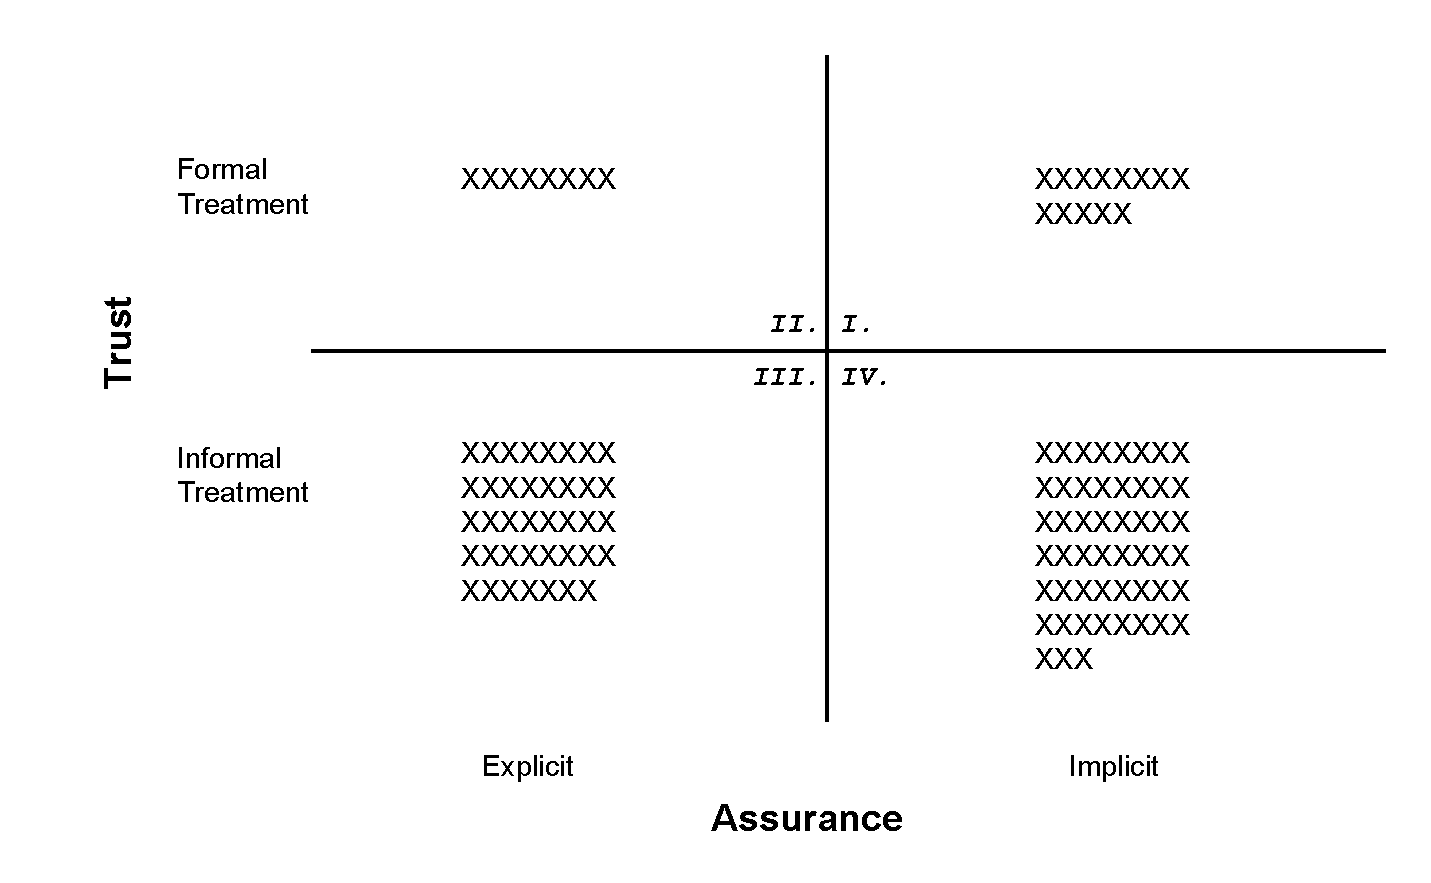
\includegraphics[width=0.6\textwidth]{Figures/Trust_vs_Assurance_Intention.pdf}
    \caption{Figure depicting how many papers that consider trust formally/informally consider intentional/unintentional assurances, \textbf{need to put actual data here, if it is a useful figure, for now the data is approximate from my memory}}
    \label{fig:trust_assurance_intention}
\end{figure}

The remainder of this survey will focus on surveying the assurance research in the formal/informal, explicit/implicit plane. Figure \ref{fig:trust_assurance_intention} shows the number of papers considered in this survey that lay in each quadrant of that plane. The quadrants are defined as:

\begin{itemize}
    \item Quadrant I. (implicit, formal) -- Use human experiments, consider a trust model, assurances are implicit (i.e. those who care about trust, but aren't designing assurance algorithms)
    \item Quadrant II. (explicit, formal) -- Use human experiments, consider a trust model, assurances are explicit (i.e. those who formally acknowledge trust from an AIA, and design assurances to affect it)
    \item Quadrant III. (explicit, informal) -- No human experiments, reference trust (or interpretability, etc..), proposed assurances are explicit (i.e. those who know that ``trust'' is important, but really just present their opinion about an algorithm that might be an assurance)
    \item Quadrant IV. (implicit, informal) -- don't reference trust, designed properties of AIA for better performance, typically reference some of the trust components such as predictability, stability, verification, but only in the context of the designer being happy.(i.e. those whose work is relevant for assurances, but they don't know it)
\end{itemize}

It is clear that much of the research that is relevant has occurred in the informal half of the plane. The aim, in order to satisfy the need for trust in AIAs, is to create more research in Quadrant II. This would mean that assurances have been formally and explicitly designed to affect user's trust. One key observation, is that there is plenty of opportunity to `move' research from Quadrants I., III., and IV. to Quadrant II. In essence this would be taking proposed methods and putting them to the test using a formal understanding of trust and appropriately designed experiments.

\subsection{Intentional and Unintentional Assurances}
    There seems to be quite a large disparity of the kinds of assurances studied by the formal and informal trust groups, as depicted in Figure \ref{fig:trust_assurance_intention}.  This is most likely due to the differing interests and skill sets. Those studying unintentional assurances seem to be more interested in investigating the human-AIA relationship. On the other hand those investigating the effect of intentional assurances are more interested in making algorithms.
    
    This figure clearly shows that there is a large space for researchers who study intentional assurances within a formal trust framework. To state the idea more clearly, this would involve actively designing assurances based on the AIA capability, and the assurance classes, and then validating these assurances in designed experiments.

    \textbf{add more stuff \ldots}


\subsection{Other stuff \ldots}

\section{A Refined View of Assurances} \label{sec:synthesis}
    From the review of Quadrants I. through IV. of the formal/informal, explicit/implicit plane, we are able to find some insights with respect to assurances and can discuss them in a more comprehensive way. Using insights from the survey a refined version of Figure~\ref{fig:SimpleTrust_one_way} can be constructed. Figure~\ref{fig:refined_assurances} incorporates all details from Section~\ref{sec:background} as well as adding some insights from the survey that give direction about the design of assurances in human-AIA trust relationships. Below we discuss the design of explicit assurances in this more detailed framework -- some of these insights might also apply to implicit assurances, but implicit assurances will not be directly discussed in this paper.

    \begin{figure}[htbp]
        \centering
        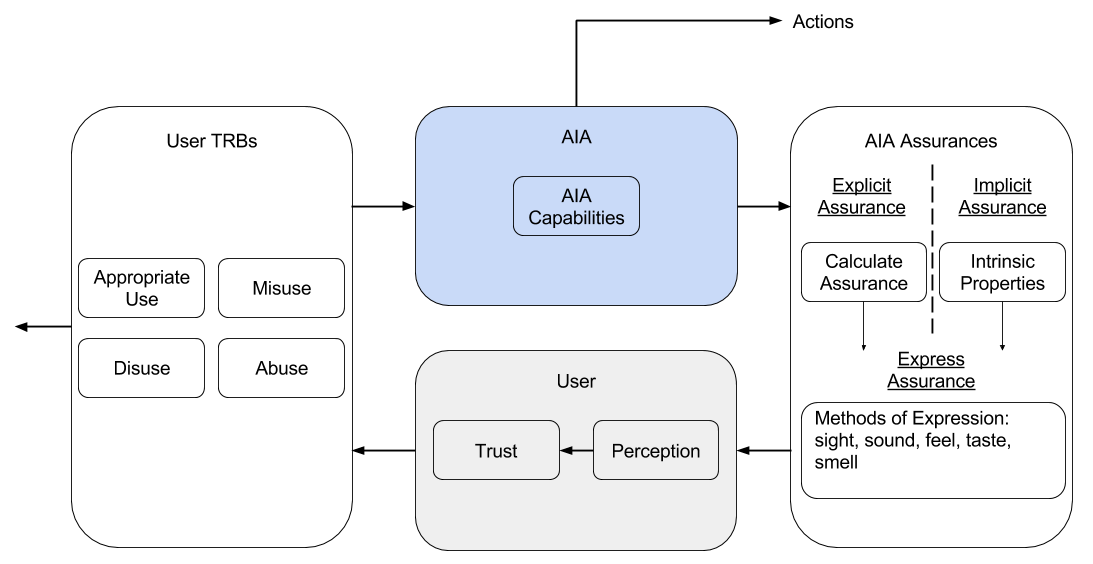
\includegraphics[width=0.9\textwidth]{Figures/RefinedTrust_one_way}
        \caption{Detailed extension of Figure~\ref{fig:SimpleTrust_one_way}. The AIA, User , and User TRBs blocks are defined as discussed in Section~\ref{sec:background} (with the exception of the `Perception' blocks added to the AIA and User boxes). The AIA Assurances box has been filled using insights from the surveyed material. The boxes that are greyed out will not be discussed in this section.}
        \label{fig:refined_assurances}
    \end{figure}

\subsection{Calculating, Designing, and Planning Explicit Assurances}
    Recall that an assurance is defined as \emph{any} behavior or property of an AIA that affects a user's trust, therefore an explicit assurance is any assurance that was consciously implemented/applied by the designer before deployment of the AIA. As such, it is possible to design assuring properties into the system a priori. It is likewise possible to design assuring behaviors into an AIA.

    From the literature, there are a couple high-level ideas that surround the calculation of assurances, these are: quantifying uncertainty, and reducing complexity. A third category that must be considered is planning strategies of assurance.

    \paragraph{Quantifying Uncertainty} Being able to quantify the different kinds of uncertainty in the AIA is necessary before attempting to express that uncertainty to a human user. There are several different kinds of uncertainty that might be considered such as uncertainty in sensing, uncertainty in planning, and uncertainty in locomotion. The general idea is that a model or method needs to be incorporated in the AIA that will represent the different kinds of uncertainty to the human user in some way. A human user could use such information to inform their trust in the `situational normality', `competence', and/or `predictability' of the AIA. 

    How have researchers approached the need to quantify uncertainty? In the surveyed literature we have seen the following main approaches. In some cases uncertainty is already represented intrinsically by the algorithms and/or models being used in the AIA. \cite{Wang2016-id} address using the built-in statistical representations of transitions and observations as the basis of quantifying uncertainty in a POMDP robot. This is an approach that has straightforward analogs in systems that use algorithms and/or models that inherently consider uncertainty.

    Models and methods that intrinsically contain or represent uncertainty are frequently available. However, even when that it is the case -- such as with POMDPs -- there are types of uncertainties that may still not be considered. \citet{Aitken2016-fb}, suggest further metrics of uncertainty beyond those intrinsically captured by a POMDP model (POMDPs contain representation of transition probabilities, and observation probabilities). Using the UGV road-network problem as an example, if the UGV calculates a distribution over possible outcomes, how favorable is that distribution? Or, given a certain road-network what kind of accuracy can be expected from the POMDP solver that the UGV is equipped with? In a similar vein \cite{Kuter2012-bv} simulated ways of breaking a plan (`counter examples'), and evaluated the system's capability of repairing the broken plan in those instances. Generally these considerations might be described as addressing `uncertainties in application', which are those uncertainties that arise when trying to apply certain algorithms and models in various environments.

    Perhaps the most obvious (but not necessarily simple) approach is to quantify the uncertainty of a classifier (regression methods have analogous approaches). \citet{Gurau2016-hs} (along with many others see Section \ref{sec:performance_prediction}) approached this problem by using a GP model for classification. In this way they, in essence, constructed a truth model from empirical training data and used that model to quantify uncertainty in different test scenarios. In contrast , \cite{Zhang2014-he} proposed quantifying the uncertainty of a classifier based solely on the input itself. They admit that this approach may have shortcomings based on the type of classifier used, but show that for many methods (i.e. algorithms that are not learning based) the method is very reasonable. Of course the methods share common drawbacks of being solely supervised learning approaches, however even in the unsupervised domain such as reinforcement learning, methods for avoiding highly uncertain (un-safe) rewards use some form of external expert knowledge (see \cite{Garcia2015-rs, Lipton2016-dq}).

    Uncertainty can be easier to assess if some kind of oracle, or reference is available for comparison. Quantifying the similarity between the empirical experience and the available reference can be a measure of uncertainty. This was illustrated by \cite{Kaipa2015-hy} who used a 3d part model to compute the confidence of a robot in identifying a part to be retrieved from a bin, by quantifying the difference between the measurements of an identified part, and those of the true part. Of course this approach loses its appeal when a truth model isn't available. This shouldn't detract from the intent of finding some kind of reference (truth or otherwise) in which the reasoning, sensing, and other processes of an AIA can be compared to evaluate uncertainty.

    The evaluation of statistical models involves a very similar concept, given a statistical model as a reference does current empirical experience support or detract from the hypothesis that the model is still valid? These ideas have been investigated by \cite{Laskey1991-mf, Laskey1995-jp, Laskey2015-gz, Zagorecki2015-qy, Habbema1976-xd, Ghosh2016-dl} who try to assess whether a statistical model is still valid. These approaches can quantify the degree to which the statistical models are still true, and this measurement can be used as an indication of uncertainty.

    Generally, the capability of quantifying uncertainty enables an AIA to be able to express assurances related to the `situational normality', `competence', and `predictability' of the system in a given situation. One might imagine that, in the UGV road-network problem, the UGV expressing high uncertainty in its plan would influence the competence component of the user's trust. Conversely, if an uncertainty measure is not available the user might take this as an implicit assurance that the AIA is perfectly confident, or based on the user's experience they might conclude that since all AIA plans have been flawed in the past, the plan of this AIA must be flawed as well.

    \paragraph{Reducing Complexity} Many researchers have attempted to remove complexity from the models and logic of the AIA to make the methods more interpretable (or comprehensible, or explainable, \ldots) to a human user. As with quantifying uncertainty, making an AIA more interpretable can also inform a user's trust regarding the `situational normality', `competence', and `predictability' of it. Perhaps \cite{Sheridan1984-kx} was the first to suggest this type of approach with respect to human-AIA relationships. Of course this presupposes that many of the methods used by AIAs are `complex' by some measure, we claim that the fact that experts are required to understand some of the methods (and even then it may not be totally possible) proves this supposition. Complexity only exists in the presence of some reference frame, which is the designer's. Generally complexity is said to increase with the number of variables, steps of reasoning, the size of data, etcetera.

    This reduction in complexity was addressed in several different ways. In practice this has been manifest in approaches as simple as finding summary statistics, or calculating averages (e.g. \cite{Muir1994-ow,Muir1996-gt}). Reducing complexity was an important goal to \cite{Aitken2016-fb} whose aim is to reduce uncertainties in models, outcomes, computational approaches, and others into a single `self-confidence' measure between $-1$ and $1$; this involves another layer of algorithms to operate on top of the various other algorithms being used in the AIA. In short, all of the approaches from Section \ref{sec:model_interp} investigate this need.

    A useful example is explaining one's research to others. When explaining to a researcher from the same field, jargon, and shared knowledge can make the explanation easier. However, when trying to explain one's research to a non-expert one must adapt the explanation to be more general and simple; this will inevitably result in the loss of detailed information, but will hopefully convey the main principles to that person. There is always a tension between a highly accurate model -- that must necessarily be complex -- and a simple yet less faithful model. 

    To this end, we find work by \cite{Ruping2006-xj}, \cite{Van_Belle2012-dt}, \cite{Ribeiro2016-uc}, and \cite{Choi2016-by} especially interesting. These methods seem promising in their attempts to make/discover/learn models with scalable interpretability based on given criteria like required depth of understanding, level of expertise, and time to gain understanding. 
    
    Research efforts such as \cite{Caruana2015-za,Huysmans2011-th,Faghmous2014-og,Venna2007-yj,Vellido2012-nm,Kadous1999-rx,Lomas2012-ie} tend to focus on creating and using models that are inherently more interpretable to humans. These efforts include constraining the feature space to be more simple, reducing dimensionality, learning more understandable features, and theoretically founding the models (i.e. interpretable science).

    One shortcoming of all of the work in Quadrants III and IV, is that they theoretically reduce the complexity of the models being used, but they have not verified this with human studies. It is quite likely that they have succeeded to some extent, but it is not clear what scale of improvements have been made. However, given the lack of a formal definition for `reducing complexity' (i.e. are there units of complexity, is it a relative or absolute scale?) it is difficult to be too critical.
    
    While it is possible that there are inherently interpretable models that can be designed that can compete with other non-interpretable models, we believe that this is not the best long-term approach to reducing complexity; this is primarily due to the lack of scalability for engineers and scientists to frequently design new algorithms. Investigating methods that generate explanations from non-interpretable models is a more promising direction. The main reason is that the idea of interpretable models is not well-defined and, in reality, doesn't exist as a single tangible goal. Instead there is a continuum of interpretability that is based on the complexity of the problem, the time required for a user to interpret (i.e. a few seconds or months of study), the expertise of the user, and others. Investigating the generation of interpretations and explanations that are user specific and model agnostic would be the best of both worlds. These ideas are much more aligned with the efforts of \cite{Ruping2006-xj} and others who seek to use models with scalable resolution and accuracy.

    \paragraph{Assurance by Design} No matter how much engineers like to think about automating everything, realistically a human will need to be involved at some level of the design for the foreseeable future, if only because the main pursuit of human-AIA trust directly involves a human. The above two approaches alone (quantifying uncertainty, and reducing complexity) can largely use existing methods, however some researchers directly engineered their methods and models in the AIA to be more meaningful to humans.

    This can be seen in \citet{Freitas2006-qo} where he considered putting a human in the learning process, he essentially modified the objective function of the learning algorithm. In essence the objective function was now based on a large set of human preferences (and biases). This kind of approach is promising, in that it can be used to encode many human qualities that cannot be easily quantified, or even explained. However, there are trade-offs that can be undesirable in many situations as well. We often use designed, objective, learning algorithms to avoid human biases. It is interesting to note that using a human in the loop can offer more interpretability to the result of a learning process, while at the same time making the learning process itself less procedural.

    \citet{Amodei2016-xi} discuss several different considerations related to AI safety (where safety can be viewed as something a user trusts to be competent and predictable in its operation, see other papers in Section~\ref{sec:safety} as well). They spend quite a bit of time discussing the situation when AI objectives don't correspond, or align, with human objectives (this is something addressed in a specific situation by \cite{Hadfield-Menell2016-ws}, also \cite{Bostrom2012-uf}). One of the main insights is that the source of discord between what humans expect and what AIAs actually do is because of poorly designed objective functions that you might refer to as myopic, or focusing on a specific objective to the extent that a human can no longer relate to the objective of the AIA (and will be correspondingly surprised by its actions). This suggests to designers that significant time may be required to design objectives that align with those of humans, this alignment will automatically make the AIA more predictable, and competent in the user's eyes. Validation and verification (from Section~\ref{sec:VV}) can have this same affect; a system that is validated and verified is a system that is assuring by design.

    Several efforts have modified standard learning approaches (like the ones discussed in the previous section) or designed their own, in such a way as to make the models/plans inherently more assuring to a human. For example \cite{Choi2016-by} intentionally restructured a neural network to pay attention to variables that users care about, in this way the outputs were rendered more interpretable. In their work \cite{Abdollahi2016-vn} added a new layer to a recommender system that only existed to contain explanations for a human user. Finally, \cite{Jovanovic2016-gw,Swartout1983-ko} 

    \paragraph{Planning Explicit Assurances} Planning assurances is critical when trying to attain desired TRBs from a human user. In this context when we say `planning explicit assurances' we mean formulating a plan for the expression of assurances over time, with the goal of more effectively and appropriately expressing assurances to a human user. Having said this we recognize that planning is not a capability available to all AIAs. In cases where AIAs don't have the ability to plan, they may be designed beforehand with some kind of static plan of assurance. Otherwise, more advanced AIAs might take into account TRBs to plan an assurance strategy to assist the human to use it appropriately.

    When planning assurances the AIA must be able to account for limitations of users, and its own limitations in expressing assurances. For example a user may not be able to understand the necessary information needed to use the AIA more appropriately. Also, the AIA may need to take a long-term strategy to teach the user, as opposed to only presenting the user with canned, static, assurances. Some of the important user considerations will be discussed further in Section~\ref{sec:express_assurances}.
    
    One must ask whether the human user can correctly process the information received. This is perhaps most easily illustrated by considering a non-expert user who cannot understand highly technical assurances regarding the AIA. However, less trivial manifestations may be troubling. This point was not directly addressed in the survey papers, but evidence of its existence were seen. For example \cite{Riley1996-qm}, and \cite{Freedy2007-sg} both observed evidence of framing effects during experiments (the tendency of a user to become too trusting once they are in the mode of trusting). This suggests the existence of other kinds of typical cognitive behaviors such as recency effects (having biased trust based on recent experiences), and the existence of bias in the perception of assurances. This will be addressed further in Section~\ref{sec:express_assurances}.

    Few papers are referenced in this subsection because it is nearly unexplored in the context of human-AIA trust relationships. However, there are several fairly new programs that are interested in this question (i.e. explainable artificial intelligence (XAI) \cite{Gunning2017-ih}, and assured autonomy)\edit{do you have references for these??? that would be good} . Assuming an AIA can give assurances there are important questions like: what is the best way to present them? How can they be adapted for different kinds of users? How can the AIA teach or tutor the human over time? This is a large gap in the current assurances landscape, answers to these questions are critical to designing more robust and effective assurances.

\subsection{Expression and Perception of Assurances} \label{sec:express_assurances}
    Expression and Perception of assurances have been combined in this section because they share several critical aspects. In designing assurances the medium, and method of expression must be selected taking into consideration the limitations of the AIA. Here medium denotes the means by which an assurances is expressed, this could be through any of the senses by which humans perceive, such as sight, sound, touch, smell, and taste. The method of assurance is the way by which the assurance is expressed. An example may help: a plot may be conveyed through sight in the typical way, or through spoken language (for example when communicating to a blind person); in this case the plot is the method, and sight or sound are the different mediums through which it can be communicated. An AIA might be limited in methods of expression because it does not have a display, or a speaker. In that situation how is the user supposed to receive an assurance?

    A designer must also consider whether a human can perceive the assurances being given. If so, to what extent is the information from the assurance transfered (i.e. how much information was lost in the communication)? A few examples include: an AIA giving an auditory assurance in a noisy room and the user not hearing it (such as an alert bell in a factory where the workers use ear-plugs), or an AIA attempting to display an assurance to a user that has obstructed vision. If an assurance is not expressed, or not perceived by the user, it is useless and has no effect. For example, an AIA may have the ability to store data about its performance, and compute a statistic regarding its reliability, but if it cannot express (or communicate) that information in some way, the information is useless.

    A user will \emph{always} have some kind of TRB towards an AIA (if only to choose to ignore the AIA). In the absence of explicit assurances the human will instead use implicit assurances to inform their TRBs. However, the general human user will not have knowledge regarding which assurances are implicit or explicit -- humans participating in research from Quadrants I and II were not aware which assurances were designed by the researchers and which weren't. Recall from Section~\ref{sec:assurances} that to a user all assurances are the same; that is to say that any property or behavior of an AIA that affects trust is an assurance, and it doesn't matter whether the assurance was designed or not (is explicit or implicit).

    The literature surveyed gives some insights into what methods and mediums of expression have been used to date. We summarize that research below.

    \paragraph{Methods:} One of the main methods by which to express an assurance is by displaying a value, such as a flow-rate, as in \cite{Muir1996-gt}. While this sounds banal it actually contains some nuanced points. The interesting part is that a value such as a flow-rate actually conveys no assurance to a human user without the human user then creating a mental model of the AIA value and inferring something like the reliability. The user's trust dimensions (`competence', 'predictability', etcetera) are then affected by this perception. This approach was also used by \cite{Wickens1999-la,Sheridan1984-kx,Hutchins2015-if} among others. It is effective, but relies heavily on the assumption that the user will create a model that is `good enough' out of the sequential display of those values.

    In a similar vein, \cite{Freedy2007-sg,Desai2012-rc,Salem2015-md} trained operators to recognize signs of failure or mannersims in different interactions with an AIA. Again, this approach relies on human users to make models that are `good enough' in order to correctly decide how to appropriately use the AIA. The main drawback of this work, and of that above is the blind reliance on users being able to make correct statistical models (of things like reliability) from noisy observations. A more ideal approach would be to design assurances that remove chances for misinterpretation because of inconsistent human models (more direct methods are discussed below).

    Another approach is to rely on the physical presence of the AIA in proximity to the human user such as investigated by \cite{Bainbridge2011-pl, Dragan2013-wd}. Generally this work looks at the communication of assurances through physical movements. In the case of \cite{Bainbridge2011-pl} this was done through the gestures of a robot that was both physically present and virtually present (through a television screen). In the case of \cite{Dragan2013-wd} this was done by users directly observing motion patterns of a robotic arm. Again, this approach utilizes the `theory of mind' where the user tries to interpret what the AIAs goals and intentions are only through correlating observations (i.e. I see the hand moving towards the cup, so the robot probably wants the cup).

    More direct methods of expressing assurances include displaying the intended movements through visual projection of a planned path \cite{Chadalavada2015-wx} -- this is subtly, but significantly different from making the user infer the intended intention. Analogously, natural language expressions (written or otherwise) attempt a more active method of expressing an assurance (such as \cite{Wang2016-id}). Finally 
    \cite{Van_Belle2013-ph, Huysmans2011-th, Hutchins2015-if}, and others investigate displaying plans and logic in different formats such as tables or trees, bar charts. These approaches attempt to remove some uncertainty regarding the human's ability to create the correct model. As humans are fond of saying ``You can't assume that I can read your mind!'', in essence more passive expressions form AIAs are relying on humans to read AIA's `minds', we can't even do that do other humans.

    Any of these methods can be more or less effective based on the task, or situation in which they are used. In \cite{Chen2014-dk,Wallace2001-fm,Kuhn1997-qc,Lacave2002-cu} they consider the ways in which uncertainty should be displayed (i.e. as a distribution, summary statistics, fractions or decimals), unsurprisingly we find that the answer is `it depends'. Things such as the experience of the user, or the nature of the information being displayed affect the user's ability to interpret the assurance.

    One final point is that there are several potential sources of explicit assurance that lack appropriate expressions, and thus cannot be effectively utilized as assurances. For example, it is unclear the best way for an AIA to express that it has been validated and verified on situations similar to the current one. Similarly, what other methods exist for communicating statistical distributions besides showing a plot (only useful for 1 or 2 dimensional distributions) or showing sufficient statistics? Investigating how assurances can be expressed in effective, and efficient ways is critical to human-AIA trust relationships.

    \paragraph{Mediums:} In this survey we saw several different mediums used to convey an assurance. Some used sight such as in \cite{Chadalavada2015-wx} where the robot gave visual feedback to a user, or in \cite{Muir1996-gt} where performance data were visible on a computer screen. Others used sight as well when communicating via natural language (i.e. \cite{Wang2016-id}) -- it is also a simple matter to convert written natural language output to spoken natural language now.
    
    The other senses (touch, smell, and taste) are not well explored in literature related to human-AIA. Generally, any human sense could be used as a medium, besides sight, and sound. Tactile feedback has been used extensively in robotics where it is called `haptic feedback' (where the user receives mechanical feedback through the robot controls). This meduim is use to create a more immersive user interface in robotics, to help users feel more connected to the robot. One can imagine smell and taste having an obvious application in the assurances of a cooking robot, other applications certainly exist as well and are open to further research.

    \paragraph{Human-like assurance:} It is generally presumed that making something more human-like will make an AIA more trustworthy. An algorithm may be human-like when it represents knowledge in a way that a human would understand, or executes logic in a way that a human can follow. A robot that is humanoid becomes more human-like in appearance (as investigated in \cite{Bainbridge2011-pl}), a system that uses natural language becomes more human-like in communication (for example in \cite{Lacave2002-cu}). Generally, since human-AIA trust relies on an interface between humans and AIAs, there must be some kind of method to make that interface more efficient. As humans are the designers of AIAs this is typically done by making an interface where the AIA becomes more human-like, by implicit or explicit means, if only when it comes time to express assurances.

    Contrasting \cite{Dragan2013-wd} and \cite{Wu2016-ei} shows that sometimes the same technique can have different effects when used in different situations. In \cite{Dragan2013-wd} the AIA is made more trustworthy by making the robot motions more human-like, whereas in \cite{Wu2016-ei} making the AIA more human-like resulted in a decrease of trustworthiness. In this case the difference came from the type of task, in the first case the robot was physically working in proximity to a human, in the other case the user was playing a competitive game against the AIA.We therefore see that making a system more `human-like' can both positively and negatively affect trust between human and AIA. \citet{Tripp2011-rx} noted that humans trust more `human-like' AIAs in more human-like ways. Perhaps in this case `human-like' applies to how difficult it is to fully understand and predict the AIA. This is definitely true with humans, one can never be sure how a human will act in given situations. Following on this idea the benefits or drawbacks of human-like characteristics are likely amplified by the risk of the situation in which being unpredictable is not conducive to increased trust.

    \paragraph{Efficiency:} Some kinds of expression are very `one-dimensional' in that they only use one medium, or method. This, again, is seen in practice by utilization of plotting a certain value over time. Because of this much of the research to date involves assurances that are not robust to loss in transfer. Because of this, exploring ways in which assurances can be robustly communicated is a clear opportunity for those trying to design assurances. This is akin to a human speaking with their voice, making facial expressions, and gestures with their hands as well; simultaneously utilizing several mediums/methods helps to ensure an assurance will be perceived correctly. Of course, repeating the same message over a thousand times is wasteful, and so enters the idea of efficiency in expression.

    Perhaps less obvious is a situation in which the user has to supplement an incomplete assurance. As a simple example, in \cite{Muir1994-ow} a simple flow-rate is provided to the user, they then supposedly create a mental model of the reliability -- based on repeated observations over time of the AIA to inform their TRBs. Creating this mental model takes time, and the model is prone to cognitive biases (discussed a bit more below). In this case the assurance is communicated slowly and indirectly.
    
    Generally, a highly efficient assurance would have precise information communicated in a way that is easy for the user to perceive, with little loss. Whereas, an inefficient assurance may be more vague, wasteful (i.e. repeating the same thing a thousand times), and susceptible to loss in communication. The likely solutions to efficiency lay in selecting appropriate methods, and mediums for expression of the assurance.

    \paragraph{Implicit and Explicit Assurances:} It is worth considering, in more detail, what implications this has on the designer. The foremost consideration is that an analysis of the interaction between the human and user need to be made in order to identify the critical assurances for a given scenario. For example, in the road network problem, an analysis might find that the most critical assurances are about the competence of the UGV's planner. In this case the designer must take time to design a planning-competence assurance.

    One difficulty arises form this approach, which is that there doesn't seem to be a way to determine what passive assurances might drown out active assurances. Following from the example above, the designer may have built an excellent planning-competence assurance, but failed to consider the effect of how the UGV appears -- it may be old, have loose panels, and rust holes. Generally, designers overlook implicit assurances (i.e. do not consider them explicitly in design) because they assume that they will have no effect (i.e. why does it matter if there are rust-holes if the UGV works?). This can stem from either: 1) ignorance of human-AIA trust dynamics, or 2) lack of identifying which assurances are most important to a human user.

    While it might be nice, it seems unreasonable, inefficient, and unwise to perform a study of \emph{every possible} assurance from an AIA to a human and then select the most important. Perhaps one way a designer might try to identify which assurances are important is to perform human studies where feedback about which characteristics of the AIA most affected the trust of the user. An approach like this would help to point out if explicit assurances are being noticed, and if there are implicit assurances that are overly influential, or that overwhelm the explicitly designed assurances. With such feedback designers would have a realistic idea about whether their explicit assurances are having the desired effect.

\subsection{Observing Effects of Assurances} \label{sec:measuring_effects}

    There are two different situations when it would be desirable to measure the effects of assurances. The first is when the designer wants to understand the effectiveness, the second would be when the AIA itself needs to measure whether assurances are effective or not. To our knowledge there has not been any work regarding the second situation where an AIA would measure response to assurances and then adapt behaviors appropriately (at least not in the trust cycle setting), however this is arguably the ultimate goal so that AIAs can themselves modify assurances to meet different needs. What does this mean practically? It seems that any method that is made for the designer to measure the effects of assurances could also be deployed into an AIA. The surveyed literature gives some insights into how that has been done to date.
   
    When it comes time to measure the effect of assurances on a human's trust there are two main approaches. The first is self-reported changes based on questionnaires, the second involves measuring changes of user's TRBs. The questionnaire approach was used extensively in many of the papers surveyed (as investigated by \cite{Mcknight2011-gv,Muir1996-gt,Wickens1999-la,Salem2015-md,Kaniarasu2013-ho} an others), questions like `how trustworthy do you feel the system is?', or `to what extent do you find the system to be interpretable?'. These kinds of questions can be useful in verifying whether the assurances are having the expected effect. It is not unreasonable to imagine that an AIA might be equipped with a method by which it can ask the user questions about their trust, process those responses, and modify assurances appropriately.
    
    However, evidence is presented in \cite{Dzindolet2003-ts} that illustrates that sometimes changes is self-reported trust do not result in changes in TRBs. From the AIAs perspective this means that --- unless the object of the assurances is to make the person's level of self-reported trust change --- the assurances are not providing any benefit. As previously discussed, the goal of assurances is to elicit appropriate TRBs from the human user. From this perspective, measuring changes in TRBs is the more objective approach to measure the effect of assurances.

    Generally researchers in the field have measured, in some way, how frequently the AIA was able to run in autonomous mode before being turned off \cite{Freedy2007-sg,Desai2012-rc}. This metric seems very reasonable, and seems to be a promising approach with some extensions. Other researchers calculated whether the user was willing to cooperate with the AIA or not \cite{Salem2015-md,Wu2016-ei,Bainbridge2011-pl}. Perhaps a better defined metric would be the likelihood of appropriate use of a certain capability by the user, albeit more difficult to formally define/calculate in different situations. As a concrete example, in the UGV road-network example there isn't really an option to `turn off' the UGV. Instead the remote operator can make decisions such as accepting a plan designed by the UGV. In this situation the effect of assurances might be measured by how likely the operator is to accept a generated plan instead of overriding it (recall that the goal may not be to have the generated plan accepted 100\% of the time, rather that it be accepted with respect to how appropriate it is in a given situation).

    Self-reports are likely the most useful when trying to understand the true effects of an assurance. Does a certain assurance, assumed to affect `situational normality', actually do that? There is space for quite a lot of research in this realm. Does displaying a specific plot actually convey  information about `predictability'? This information can be used to inform the selection of the methods of assurance.

    In practical application (such as in the UGV road-network problem), the user, and the human-AIA team, care more about whether TRBs are appropriate or not. It doesn't help if an assurance helps the user feel that the AIA is more competent, if the user doesn't treat the AIA any differently than before the assurance. This assumes that it is possible for appropriate TRBs be measured in the first place. For example, if appropriate behavior is for the user to verify a sensor reading, can the AIA perceive that? In that situation perhaps the easiest approach would be to ask the user, but what if the user lied? Is there a way to verify the TRB is actually appropriate? This is something that has gained notoriety with autonomous cars, where the car can drive itself, but the user still needs to sit in the driver's seat and be attentive just in case the vehicle cannot perform correctly. We claim that it is as important to design methods of perceiving appropriate (and inappropriate) TRBs as it is to design assurances. 
%
% \subsection{The Imprecise Nature of Assurances} \label{sec:imprecise_nature}
    % Due to the nature of trust (and humans in general), a single assurance might be targeted at influencing the competence dimension of trust, but it may also have effects on other dimensions. As an example an assurance that targets predictability may also have an affect on the probability of depending.
%
    % Besides being difficult to separate effects on a single user, individual users are different as well. Thus no assurance will have an identical effect when given to two separate users. This makes it difficult to have precise effects on user trust behaviors.
%
    % One might attempt to mitigate this uncertainty by using expressions that are more precise than others, such as displaying a probability distribution rather than on a maximum likelihood. This gets into some considerations about how the presentation of information affects the ability of a human to understand.

The issues of user trust in AIAs and appropriate deployment/use of AIAs have become very prominent.  Assurances are the method by which AIAs can influence humans to trust and (more importantly) \emph{use} them appropriately. We have presented here a definition, case for, and survey of algorithmic assurances in the context of human-AIA trust relationships. A formal treatment of this topic is necessary because the ecosystem of AIAs is evolving more rapidly than ever before; consequently, previous informal approaches to designing algorithmic assurances are insufficient. 

This survey was performed, to some extent, from a standpoint of designing intelligent unmanned vehicle systems that must work in concert with a human supervisor. However, the theoretical framework and categorization of assurances is meant to be generally applicable to a broad range of AIAs. A major motivation for this survey was the observation that there are many researchers in different but related domains such as human factors, robotics, machine learning, artificial intelligence, and others who are (unknowingly) working along different parts of the same human-AIA assurance spectrum. It is important for members of each community to recognize this, so that research efforts can be  methodically organized to answer related open questions in this important area. Assurances have historically been ignored from a practical standpoint, and are the least understood component of human-AIA trust relationships. There have been many researchers who have recognized the concepts behind assurances, but no detailed definitions have been given until now.

There are three main contributions from this work: 1) we have drawn from multiple bodies of research in order to fill in the missing details for the human-AIA trust cycle (Fig.~\ref{fig:SimpleTrust_one_way}) and to formally define assurances within this cycle; 2) we present a classification of assurances in Sec.~\ref{sec:assurances}; 3) we identify an `assurance integration continuum' shown in Fig.~\ref{fig:assurance_continuum}. On that continuum seven different classes of algorithms were identified. Practitioners can use these classes to select and design assurances for AIAs. Given the material provided herein, those who design assurances should have the tools required to approach design and future research from a solid theoretical foundation.

A final important and sobering takeaway is that there is not a single `silver bullet' algorithmic assurance that will perform the best in all situations. 
Given enough time, it is quite possible that highly specialized assurances could be designed for many situations. Even so, we warn that, for the research and design of assurances to be sustainable in the current environment of fast-paced development of new technology, it is important to consider approaches that are as principally grounded as possible, in order to be more easily used with yet-to-be-invented methods for implementing various AIA capabilities. We have identified many future opportunities for research on AIA assurance design and their influence on human trust, and hope researchers will begin looking outside of their own disciplines to discover, design and formally test new tools and ideas for assurance design and implementation. The framework presented here should unify research efforts by providing a common taxonomy in relation to human-AIA trust relationships. We believe it will help researchers see the field from a larger perspective, classify the type of research they are performing, and consider the greater implications of their work. The field of algorithmic assurances has an abundance of avenues for new and challenging research, and we encourage researchers to pursue them.


\bibliographystyle{ACM-Reference-Format}
\bibliography{References}
\end{document}
